\subsubsection{Overview}
During the NASA Lunabotics competition, visual fiducial markers may be placed above the collection
bin in order to assist the robot in finding and navigating to the bin.
The visual tracking subsystem implements detection and range finding for several fiducial markers
at a time.
The AprilTag system of fiducial markers was chosen for the implementation of the visual tracking
subsystem, specifically the 36h11 family of tags, due to its robustness even at long distances, as
well as a widespread userbase in robotics and computer vision applications.
The StereoLabs ZED 2 stereo camera, which is used to collect 3D point cloud data for the pathfinding
subsystem, is used in conjunction with the OpenCV computer vision API to detect the AprilTag targets.
A single camera view is used to detect the tags, and then stereo vision is used to determine the
distance to the tag once it has been located.
\begin{figure}[htbp]
    \centering
    
\includegraphics[width=50mm]{april}
    \caption{
        Example of an AprilTag fiducial target
    }\label{fig:april}
\end{figure}

\begin{figure}[htbp]
    \centering
    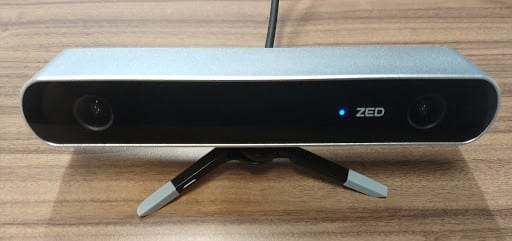
\includegraphics[width=50mm]{zed}
    \caption{
        The ZED 2 stereo camera
    }\label{fig:zed}
\end{figure}

\newpage

\subsubsection{Test Plan}
The visual tracking subsystem is verified through manual testing.
Testing is conducted by setting up a computer with the ZED 2 plugged in and placing AprilTag markers,
either printed or on a computer screen, in front of the camera.
The software should detect any targets in view and determine the distance to any target placed
greater than 50cm away from he camera (as the device cannot accurately measure range within 50cm).
For thorough results, multiple targets should be tested at several different ranges and angles,
and in different lighting conditions.
A tape measure can be used to verify the accuracy of the range measurements.

\subsubsection{Test Results}
The vision subsystem was able to successfully identify multiple targets and accurately measure the
distance to within several cm and at very wide viewing angles.
In good lighting conditions, the device was able to detect targets at a range of up to 2.6m,
while in very poor lighting it could detect targets up to 2m away.
Due to USB bandwidth limitations of the computer used in testing, the test was run at a resolution
of only 1344x376.
With a faster USB port, the ZED camera can run at resolutions of up to 2K,
which should significantly increase the target detection range.

\newpage

\begin{figure}[!htbp]
    \centering
    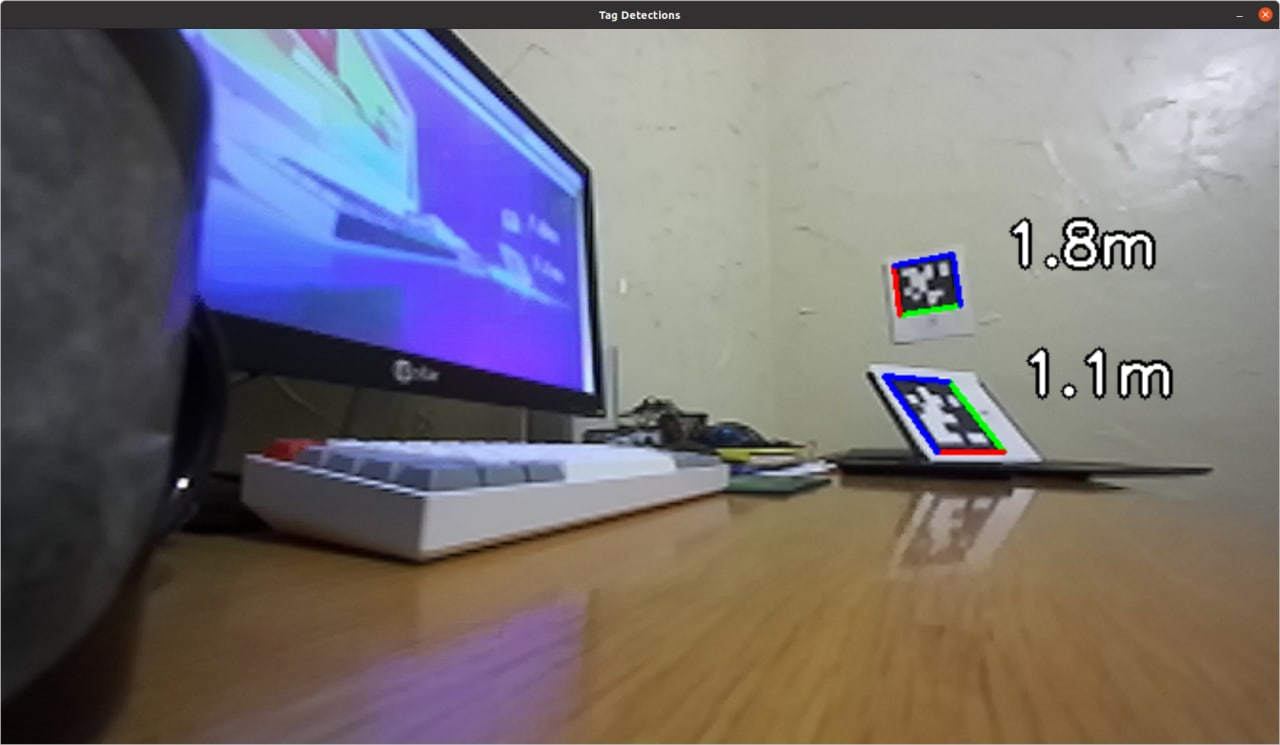
\includegraphics[width=150mm]{glt}
    \caption{
        Test in good lighting conditions
    }\label{fig:glt}
\end{figure}

\begin{figure}[!htpb]
    \centering
    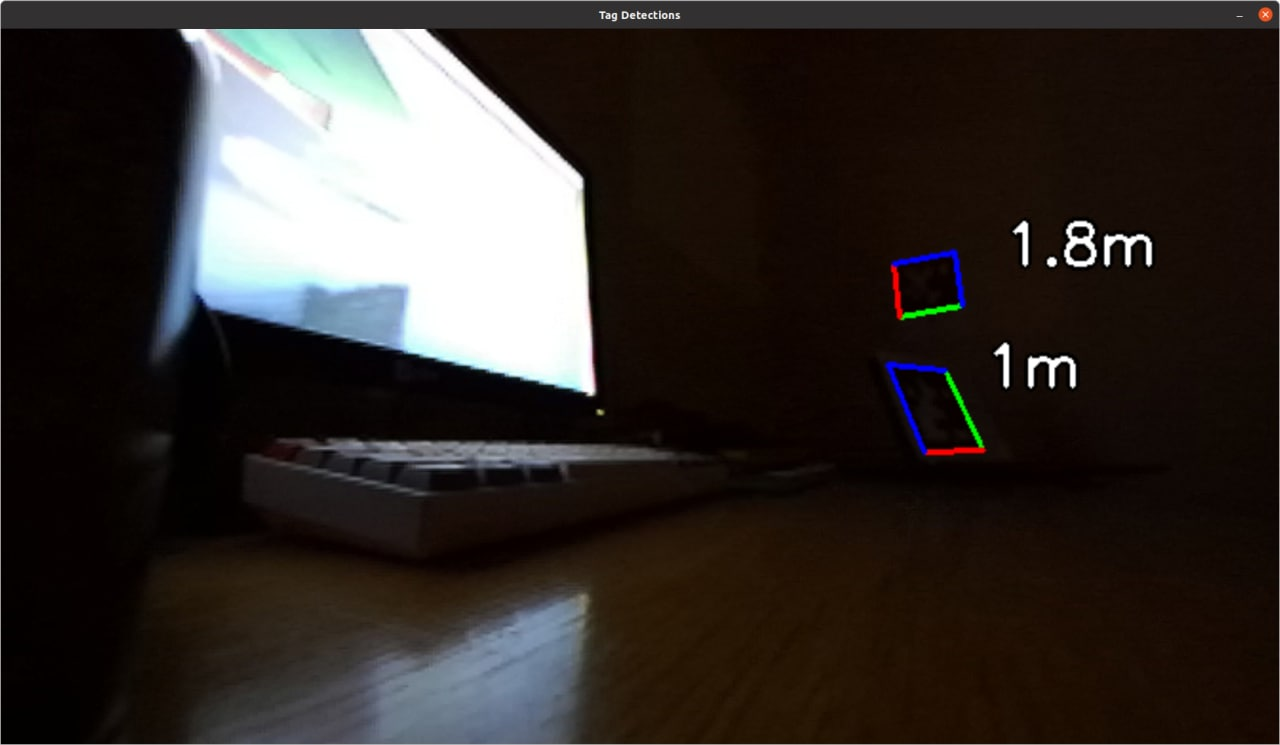
\includegraphics[width=150mm]{plt}
    \caption{
        Test in poor lighting conditions
    }\label{fig:plt}
\end{figure}
\newpage